%\documentclass{beamer}
%\usetheme{Pittsburgh} 
\documentclass{scrartcl}

\usepackage[utf8]{inputenc}
\usepackage{default}
\usepackage[procnames]{listings}
\usepackage{graphicx}
%\usepackage[toc,page]{appendix}
\usepackage{caption}
\usepackage{hyperref}
\usepackage{color}
\usepackage{pdfpages}


%Bibliogrpahy?
\usepackage{bibentry}
%\nobibliography*
%\bibentry{ }


\begin{document}

\title{Assignment No. 6}
\subtitle{}
\author{
  Quignon, Christophe \\
  %Familyname, Name
} 
\date{\today}


\maketitle

\section{Read chapter 4 from Haykin's book
}
\begin{enumerate}
\addtocounter{enumi}{6}
\item Output representation and decision rule
	\begin{itemize}
	\item For an M-Class specification NN we need m outputs.
	\item The question now is how to decide which outputs generate which classification
	\item This is easy if the output is binary
	\end{itemize}

\item Computer experiment
	\begin{itemize}
	\item Classify two overlapping Gaussian distribution is not trivial
	\item The Bayesian decision boundary calculate how likely it is for every measurement to belong to one of the Gaussian and then assigns according to higher likelihood
	\item In Experimental Determination varies several parameter to determine the optimal NN setup. Thos parameters are:
		\begin{itemize}
		\item Number of hidden neurons
		\item Learning rate parameter
		\item Momentum constant
		\end{itemize}
	\item The optimal number of hidden neurons can be varied to optimize the NN
	\item The Training Set size and the Number of epochs are varies (But their product has to stay the same) while we are looking for an optimal Mean Square error and probability of correct classification
	\item The optimal Learning Momentum constant can be optimized by three definitons:
		\begin{itemize}
		\item Local convergence of the minimum error with as few epochs as possible
		\item Conversion to a global minimum \dots
		\item Convergence to the best generalization \dots
		\end{itemize}
	\item Evaluation of Optimal Network Design is done according to three parameters:
		\begin{itemize}
		\item Decision boundary
		\item ensemble-averaged learning curve
		\item probability of correct classification
		\end{itemize}
 	\end{itemize}
	
\addtocounter{enumi}{3}
\item Generalization
	\begin{itemize}
	\item A NN is generalizing well, if the categorization of input not in the training set is done good. 
	\item To do so, the NN must not overfit the values
	\item one selection criteria to choose a function for the NN is Occams razor
	\item The generalization is influences by three factors:
		\begin{itemize}
		\item The size of the training set
		\item The Architecture
		\item The physical complexity of the problem
		\end{itemize}
	\item In practice either the architecture or the training set size is fixed
	\end{itemize}
	
\item Approximation functions
	\begin{itemize}
	\item Two layers can map any boolean function
	\item Three layers can map any function
	\item The numbers of layers as given above may not be optimal
	\item Function approximation can be measured by two factors:
		\begin{itemize}
		\item Accuracy of best approximation
		\item Accuracy of empirical fit of the approximation
		\end{itemize}
	\item The curse of dimensionality also applies to NN
	\item As a practical consideration, local optima are often the goal
	\end{itemize}
	
\item Cross-Validation
	\begin{itemize}
	\item In cross validation, a fraction of the sample set is not trained but used for validation.
	\item the validation set must not be in the training set. Otherwise the validation is not valid
	\item The split can be choosen by different measures:
		\begin{itemize}
		\item If the output is less complex than the output, the crossvalidation is insensitive to the split
		\item A single fixed split works fine for a wide range of target functions
		\end{itemize}
	\item The Cross validation may also lead to an early stop of learning
	\item Adding noise may improve generalization
	\item One may also choose a different validation subset for several trials
	\end{itemize}

\addtocounter{enumi}{1}
\item Virtues and Limitations of Back-Propagation
	\begin{itemize}
	\item BP is simple to compute locally
	\item It is gradient based
	\item BP NNs are often designed as a biological metaphor (not always justified)
	\item Local computation permits graceful degradation
	\item It favours parallel computation
	\item It is useful for feature detection
	\item Is works fine for function approximation
	\item It is computationally efficient
	\item It s robust
	\item The convergence is proven but sometimes slow
	\item It may get stuck in local minima
	\item It scales well
	\end{itemize}
	
\item Accelerated Convergence
	\begin{itemize}
	\item There are four mayor heuristics to accelerate convergence:
		\begin{itemize}
		\item Every node should have its own learning rate
		\item Every learning parameter should vary from time to time
		\item If the gradient does not change, learning rate should increase
		\item If the gradient changes signs, the learning rate should decrease
		\end{itemize} 
	\end{itemize}
\item Convolutional Networks
	\begin{itemize}
	\item Convolutional networks work on images and are invariant to distortions of the images
	\item Convolutional Networks can also be used for:
		\begin{itemize}
		\item Feature Extraction
		\item Feature mapping
		\item Subsampling
		\end{itemize}
	\item The Convolutional NN usually has five layers that alternate between convolution and subsampling.
	\end{itemize}
\end{enumerate}

\section{In this exercise you are going to do both binary and multiclass classification on real
world data.
}
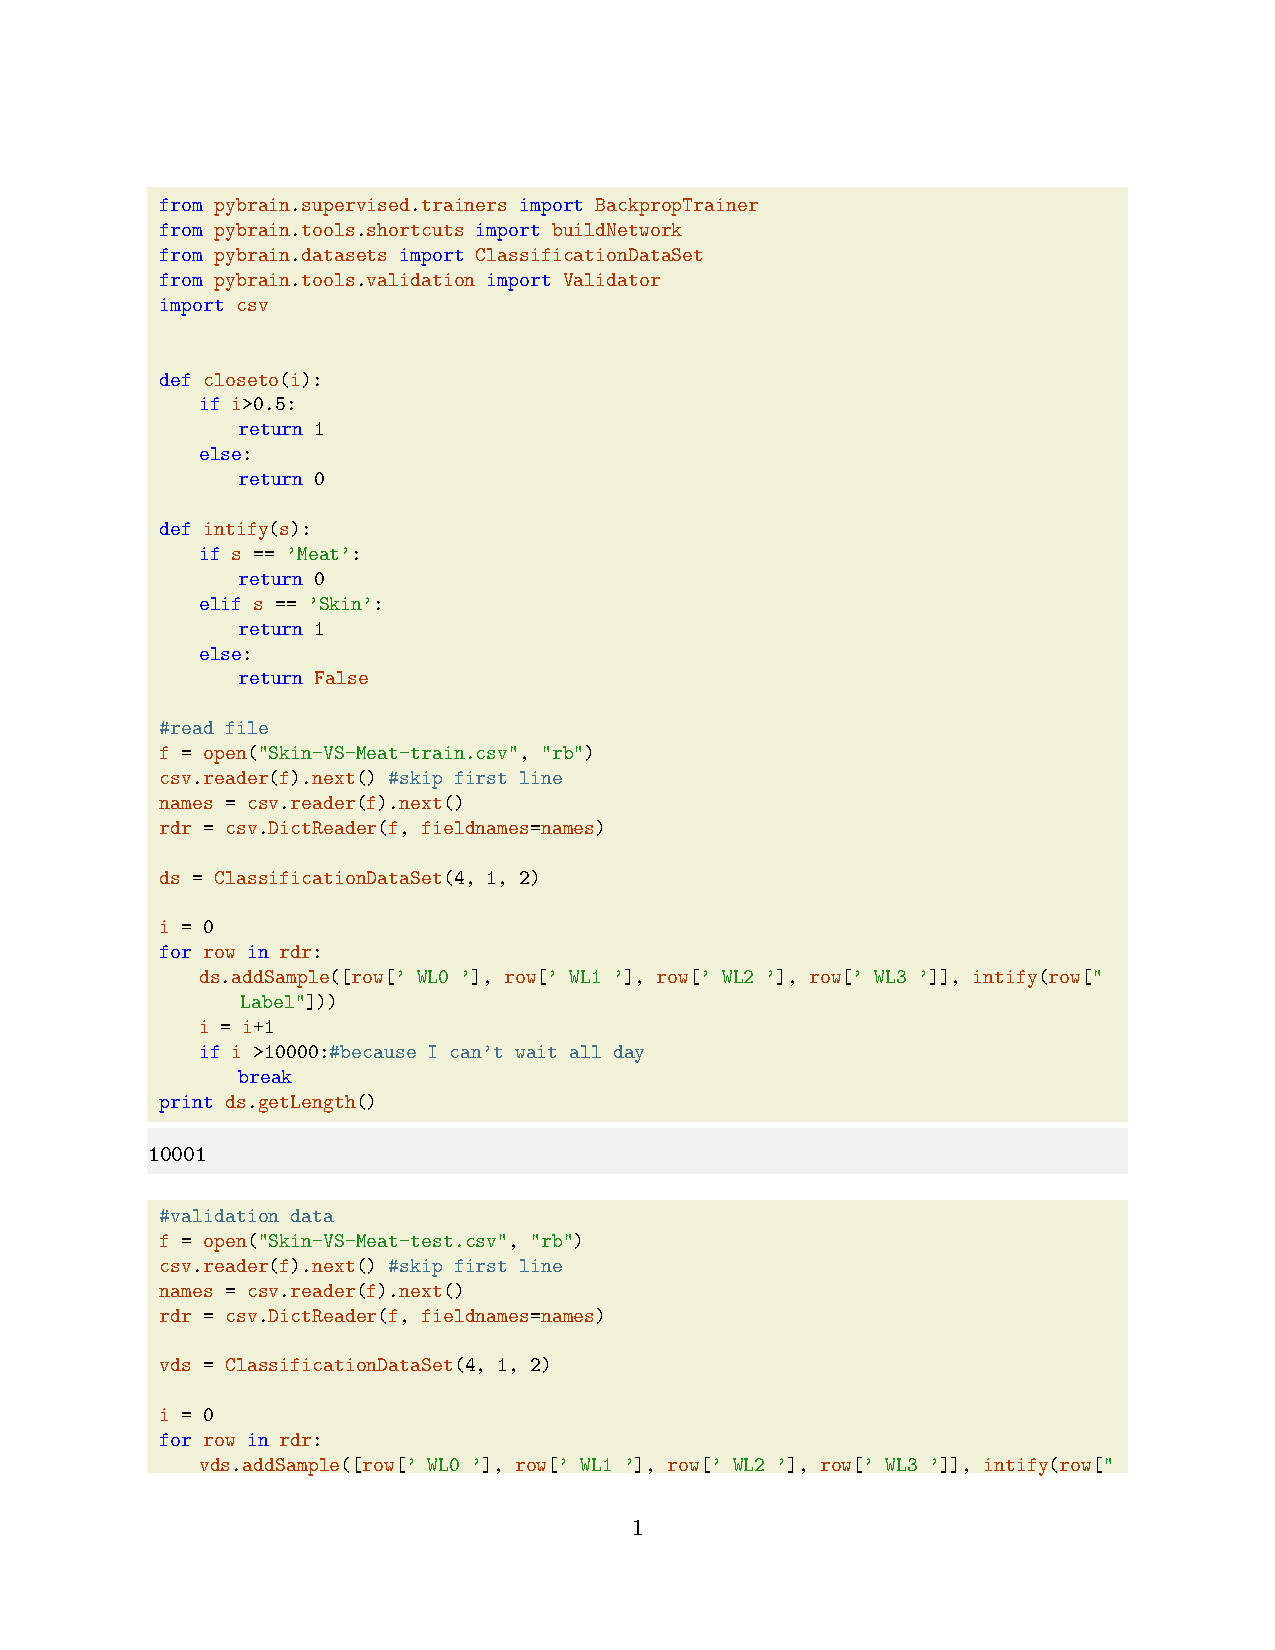
\includepdf[pages={1-},scale=1]{Ex6.pdf}

%CONTENTS
%NOTES


%COPY AND PASTE FROM HERE

%\begin{enumerate}
% \item 
%\end{enumerate}

%\hyperref{link}{text}

%\begin[Language=Python]{lstlisting}
%#PYTHON CODE HERE
%\end{lstlisting}

%\lstinputlisting[Language=Python]{ }

%\begin{figure}
% \center
% \includegraphics[width= cm]{ }
% \caption{}
%\end{figure}

%BIBLIOGRPAHY?
\bibliographystyle{plain}%amsalpha
\bibliography{Top30.bib}
%\bibentry{}

\end{document}
